\section{Contexto}
\begin{frame}
\frametitle{Contexto}

O contexto dessa tese prev� o cen�rio de manuten��o com o uso de realidade aumentada como uma ferramenta
 para aux�lio nas tarefas rotineiras. Algumas vari�veis devem ser
 consideradas para garantir a viabilidade de implanta��o da abordagem:
\begin{itemize}
\item Velocidade de reconhecimento;
\item Qualidade do reconhecimento;
\item Invari�ncia � par�metros ambientais.
\end{itemize}

\end{frame}

\subsection[Cen�rio]{Cen�rio}
\begin{frame}
\frametitle{Cen�rio}

 Como caso de uso ser� adotado a janela de inspe��o frontal, como mostrado na
 imagem~\ref{fig:ERJ190}, localizada na aeronave Embraer ERJ-190. 
 
\begin{figure}[h!]
\centering
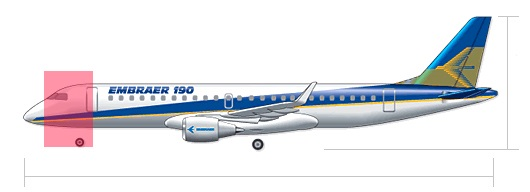
\includegraphics[scale=0.4]{images/ERJ190}
\caption{Posicionamento da LRU}
\label{fig:ERJ190}
\end{figure}



\end{frame}